%% this is necessary stuff to make the document compile:
\documentclass[reqno,11pt]{amsart}
\usepackage{amssymb, amsmath}
\usepackage{colordvi,verbatim,hyperref}
\usepackage{graphicx}
\usepackage{amsthm}

\usepackage[dvipsnames]{xcolor}
\usepackage{tikz}
\usetikzlibrary{positioning}

%% this is for making margins the way I like them:
\headheight=8pt
\topmargin=0.375truein
\topmargin=-0.2truein
\textheight=9truein   \textwidth=6.3truein
\oddsidemargin=.1in \evensidemargin=.1in

%%this is to create new math commands. In other words, since I use theta^hat in equations a lot, I made a shorthand for it. So now instead of using $\hat\theta$ every time, I can just write $\thhat$. 
\newcommand{\Q}{{\mathbb{Q}}}
\newcommand{\N}{{\mathbb{N}}}
\newcommand{\R}{{\mathbb{R}}}

\pagestyle{plain}


\date{\today}%7 Feb 2014}

\begin{document}
\title{An Analogy of Fokker-Planck Approximation Methods}
\author{Trenton Gerew}

\maketitle
	\begin{figure}[h!]
		\centering
		
		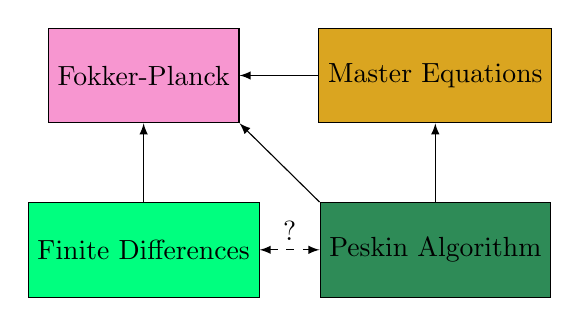
\begin{tikzpicture}
			% F-P
			\node [draw,
				fill=Rhodamine!50,
				minimum width=2cm,
				minimum height=1.2cm
				] (fp) at (0,0) {Fokker-Planck};
			
			% Master Equations
			\node [draw,
				fill=Goldenrod,
				minimum width=2cm,
				minimum height=1.2cm,
				right=1cm of fp
				] (me) {Master Equations};
				
			% Finite Differences
			\node [draw,
				fill=SpringGreen,
				minimum width=2cm,
				minimum height=1.2cm,
				below=1cm of fp
				] (fd) {Finite Differences};
				
			% Peskin Algorithm
			\node [draw,
				fill=SeaGreen,
				minimum width=2cm,
				minimum height=1.2cm,
				below=1cm of me
				] (pa) {Peskin Algorithm};
				
			% Arrows
			\draw[-latex] (me.west) -- (fp.east);
			\draw[-latex] (fd.north) -- (fp.south);
			\draw[-latex] (pa.north) -- (me.south);
			\draw[-latex] (pa.north west) -- (fp.south east);
			\draw[latex-latex,dashed] (fd.east) -- (pa.west)
				node[midway,above]{?};
		
		\end{tikzpicture}
		
		\caption{Approximation methods and their relationships to the Fokker-Planck equation. \label{fig:relationships}}
	\end{figure}

	The probability density $\rho (x,t)$ evolves according to the Fokker-Planck equation
	\begin{equation} \label{eq:f-p}
		\partial_t \rho (x,t) = \partial_x \left( \rho (x,t) \partial_x \phi (x) + \partial_x \rho (x,t) \right)
	\end{equation}
	where $\phi (x)$ is the potential energy.
\end{document}